\documentclass[preprint,proceedings]{rmaa}
\usepackage{wasysym}


%%%
%%% Define any personal macros here
%%% 

% These are some I use in typesetting example code
\newcommand{\bs}{\textbackslash}
\newcommand{\CS}[1]{\texttt{\textbackslash #1}}
% roman subscripts in math
\newcommand{\Sub}[1]{_\mathrm{#1}}
% a command to specify possible linebreak points in an email address 
\newcommand{\D}{\discretionary{}{}{}}

%%%
%%% Article preamble commands (title, authors, abstract, etc.) 
%%% None of these produce any output themselves, they just set things 
%%% up for \maketitle
%%%

% This is only used for making the header for the preprint version
\SetYear{2016}
\SetConfTitle{XV LARIM}

% Please use mixed case here, since this title gets propagated onto
% the web page, ADS entry, etc. 
  \title{Observational evidence of star formation stpchasticity in the CALIFA dataset}
 \author{Nicol\'as Romero-D\'iaz\altaffilmark{1}, J. E. Forero-Romero\altaffilmark{1}}

\altaffiltext{1}{Departamento de F\'isica, Universidad de los Andes, Cra 1 18A-10, Bloque Ip, Bogot\'{a}, Colombia.}



  % List of authors used to construct table of contents
  \listofauthors{Nicol\'as Romero-D\'iaz, J. E. Forero-Romero}
  % Each author in Surname, Initials format, used in generating Author
  % Index entries.
  \indexauthor{Romero-D\'iaz, N. }
  \indexauthor{Forero-Romero, J. E.}


% No \abstract or \resumen for poster papers

% Keywords must be from the standard list and in alphabetical order. 
\addkeyword{CALIFA survey}
\addkeyword{Equivalent width}
\addkeyword{Star formation rate}
\addkeyword{Stochasticity}



%%%
%%% Beginning of document proper
%%%
\begin{document}
% Typeset article header
\maketitle 
%%%Resumen en Español%%%
\boldabstract{En este trabajo estudiamos datos espectrales publicados por el grupo del sondeo CALIFA. Encontramos que al analizar regiones de baja formaci\'on estelar (SFR) se observan fluctuaciones de la raz\'on H$_{\alpha}/$H$_{\beta}$ que no son completamente explicadas por efectos de polvo interestelar. Proponemos que esta fluctuaci\'on detectada es debida a la influencia de procesos estoc\'asticos, los cuales han sido cuantificados en simulaciones anteriores.}

%%%Abstract%%%

\boldabstract{In this work, we study spectral data published by the CALIFA survey. When analyzing regions of low star formation rate (SFR) we find fluctuations of the H$_{\alpha}/$H$_{\beta}$ which are not fully explained by interstellar dust effects. We propose that the detected fluctuation is due to the influence of stochastic effects, which have been quantified in previous simulations.}\\

Using the CALIFA data published by PIPE3D\citep{PIPE3D}, we study the ratio between the H$_{\alpha}$ and H$_{\beta}$ emission line intensities. According to simulations, regions of low SFR are susceptible to stochastic effects due to irregular bursts of star formation as well as finite sampling in mass and time. The combination of these factors is believed to cause fluctuation of emission line intensities\citep{Forero}. With the CALIFA data, we make a histogram of the H$_{\alpha}/$H$_{\beta}$ value distribution, discriminating data according to high SFR $\left(>1.89\times10^{-1} \, \mathrm{M_{\astrosun}yr^{-1}}\right)$, low SFR $\left(< 2.99\times10^{-2} \, \mathrm{M_{\astrosun}yr^{-1}}\right)$ and a region in between. This provides a visualization of emission line fluctuations according to different SFR.

\begin{figure}[h!]
\centering
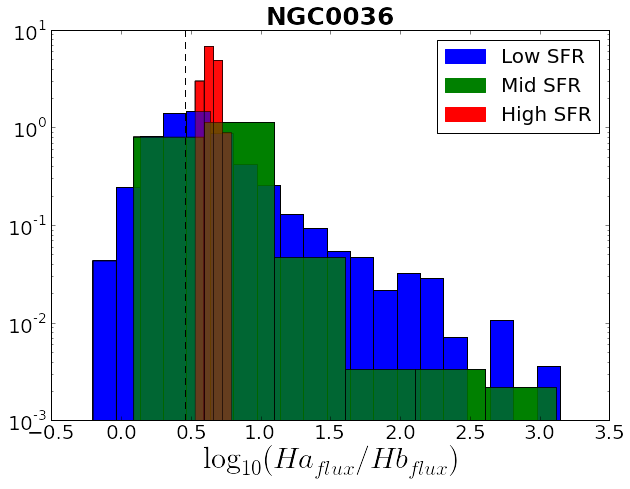
\includegraphics[width=0.5\textwidth]{HIST_FINAL.png}
\label{fig1}
\caption{Distribution of H$_{\alpha}/$H$_{\beta}$ values according to high, mid or low SFR.}
\centering
\end{figure}

In\citep{Forero}, fluctuations of the Ly$_{\alpha}$ EW where also detected, in order to study effects on EW, we analyse the OII EW. Once again, we discriminate data according to the previous high, mid and low SFR and check if the distribution of the EW varies according to SFR.

\begin{figure}[h!]
\centering
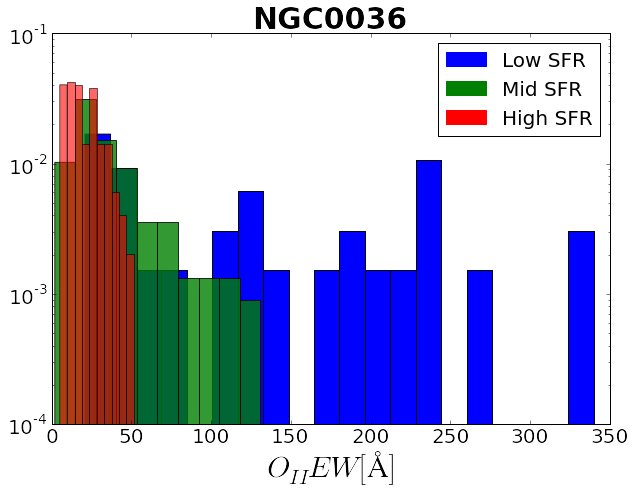
\includegraphics[width=0.5\textwidth]{OIIEW_FINAL.png}
\label{fig2}
\caption{Distribution of OII EW values according to high, mid or low SFR.}

\centering
\end{figure}

Despite lacking dust effect corrections, we can put forth stochasticity as a significant influence in low SFR regions. This is because dust is not as abundant in low SFR regions as it is in high SFR regions. Furthermore, interstellar reddening causes fluctuation in only one direction, which is not the case for the data. In our results, data associated with low SFR values is clearly more broadly distributed than at higher SFR. A fitting procedure was performed on the observed distributions and was found to follow the behaviour described in simulations\citep{Forero}.  \\
 
\begin{thebibliography}
\bibitem{Forero} J. E. Forero-Romero and M. Dijkstra. “Effects of star-formation stochas-ticity on the Lyα and Lyman continuum emission from dwarf galaxiesduring  reionization”.  In:  428  (Jan.  2013),  pp.  2163–2170.doi:10.1093/mnras/sts177. arXiv:1206.0726
\bibitem{PIPE3D} S. F. S\'anchez et al. “Pipe3D, a pipeline to analyze Integral Field Spec-troscopy Data: II. Analysis sequence and CALIFA dataproducts”. In:52 (Apr. 2016), pp. 171–220. arXiv:1602.01830 [astro-ph.IM].

  
\end{thebibliography}

\end{document}